\documentclass[12pt]{article}
\usepackage[arabic]{babel}
\usepackage[utf8]{inputenc}
\usepackage{amssymb, amsmath}
\usepackage{geometry}
\usepackage{graphicx}
\usepackage{wrapfig}
\usepackage{caption}
\usepackage{ulem}
\usepackage{xcolor}
\usepackage{polyglossia}
\usepackage{tikz}
\usetikzlibrary{arrows.meta, positioning, shapes}
\setdefaultlanguage{arabic}
\setotherlanguage{english}

% Font and layout settings
\newfontfamily\arabicfont[Script=Arabic,Scale=1.2]{Amiri}
\geometry{top=2cm, bottom=2cm, left=2cm, right=2cm}

% Colors
\definecolor{titleColor}{HTML}{800000} % Maroon for titles
\definecolor{sectionColor}{HTML}{4682B4} % SteelBlue for sections
\definecolor{textHighlight}{HTML}{DAA520} % Goldenrod for highlights
\definecolor{backgroundColor}{HTML}{F0F8FF} % AliceBlue background
\definecolor{emphasisColor}{HTML}{228B22} % ForestGreen for emphasis

\begin{document}

% Title
\begin{center}
    {\Huge\textbf{\color{titleColor} الفكي قيلي: العالم المتجول في شمال السودان}}  
    \vspace{0.5cm}
\end{center}

\section*{\color{sectionColor} النسب العائلي}
\begin{itemize}
    \item \textbf{بابكر، مالك، عثمان، علي، الشيخ، محمود}
    \item \textbf{الفكي قيلي، مالك، مدني، عبدالرحمن، أبو القاسم، حميدة، حمد، حميدة، سراج، مصباح، سليم، رباط، غلام الله، عائد}
    \item \textbf{مقبول، أحمد الزيلعي، محمود، هاشم، مختار، علي العسكري، محمد، أبو القاسم، محمد الزامل، إسماعيل}
    \item \textbf{أحمد التقي، محمد النقي، علي الرضا، موسى الكاظم، جعفر الصادق، محمد الباقر، زين العابدين علي، الحسين، بن علي كرم الله وجهه، والسيدة فاطمة الزهراء بنت رسول الله صلى الله عليه وسلم}
\end{itemize}

\section*{\color{sectionColor} نبذة تاريخية عن الفكي قيلي}
هو \textbf{\color{emphasisColor} الفكي قيلي} صاحب القبة الموجودة حاليًا في \textbf{العفاض}، حيث درس الفقه وحفظ القرآن على يد جده \textbf{مدني}.  

في فترة الحكم التركي، طلب الأتراك من جده الفكي قيلي الحضور إلى تركيا ليكون ضمن علماء البلاط التركي وديوان الإفتاء، لكنه فضل البقاء في \textbf{السودان}، متجولًا في شمال البلاد لنشر العلوم الدينية وتعليم الفقه في مناطق عديدة.



\begin{wrapfigure}{r}{0.4\textwidth}
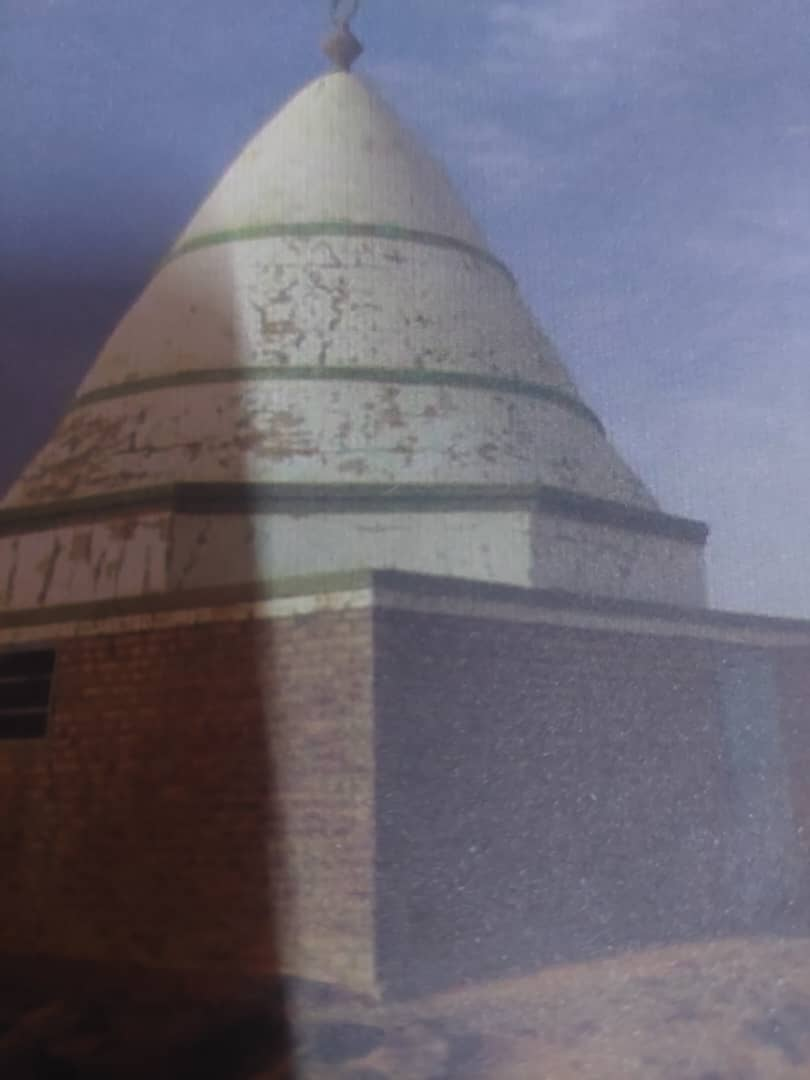
\includegraphics[width=0.4\textwidth]{y5.jpg}
\end{wrapfigure}



\begin{english}
\begin{center}
{\Huge\textbf{\textcolor{titleColor}\english{The Role of Sufi Orders in Sudan }}} \\
\end{center}

The Sufi orders have played a significant cultural and economic role in the lives of people in Sudan. Thanks to them, the social fabric has held together for centuries, achieving national unity through their influence. An example of this is our great ancestor, Sheikh Gili Wad Malik, who inherited the Qadiri Sufi lineage from his grandfather, Hamida the Great, the disciple of Gulamullah bin A'id. Tribes gathered around them, life stabilized, and social harmony was achieved. How much we need today to draw inspiration from this heritage and connect our turbulent present with our bright past.

\end{english}

\vspace{.2cm}

\begin{arabtext}
{ \hspace{.1cm} للطرق الصوفية دور ثقافى واقتصادى كبير فى حياة الناس فى السودان، وبفضلهم تماسك النسيج الاجتماعى لقرون طويلة، وتحققت الوحدة الوطنية من خلالها. ومثال لذلك جدنا الاكبر الفكى قيلي ود مالك الذى ورث السجادة القادرية من جده حميدة الكبير حفيد غلام الله بن عائد. حولهم التفت القبائل واستقرت الحياة، وتحقق السلم الاجتماعى. ما احوجنا اليوم ان نستلهم التراث ونربط حاضرنا المضطرب بماضينا المشرق.}
\end{arabtext}
\begin{wrapfigure}{r}{0.4\textwidth}
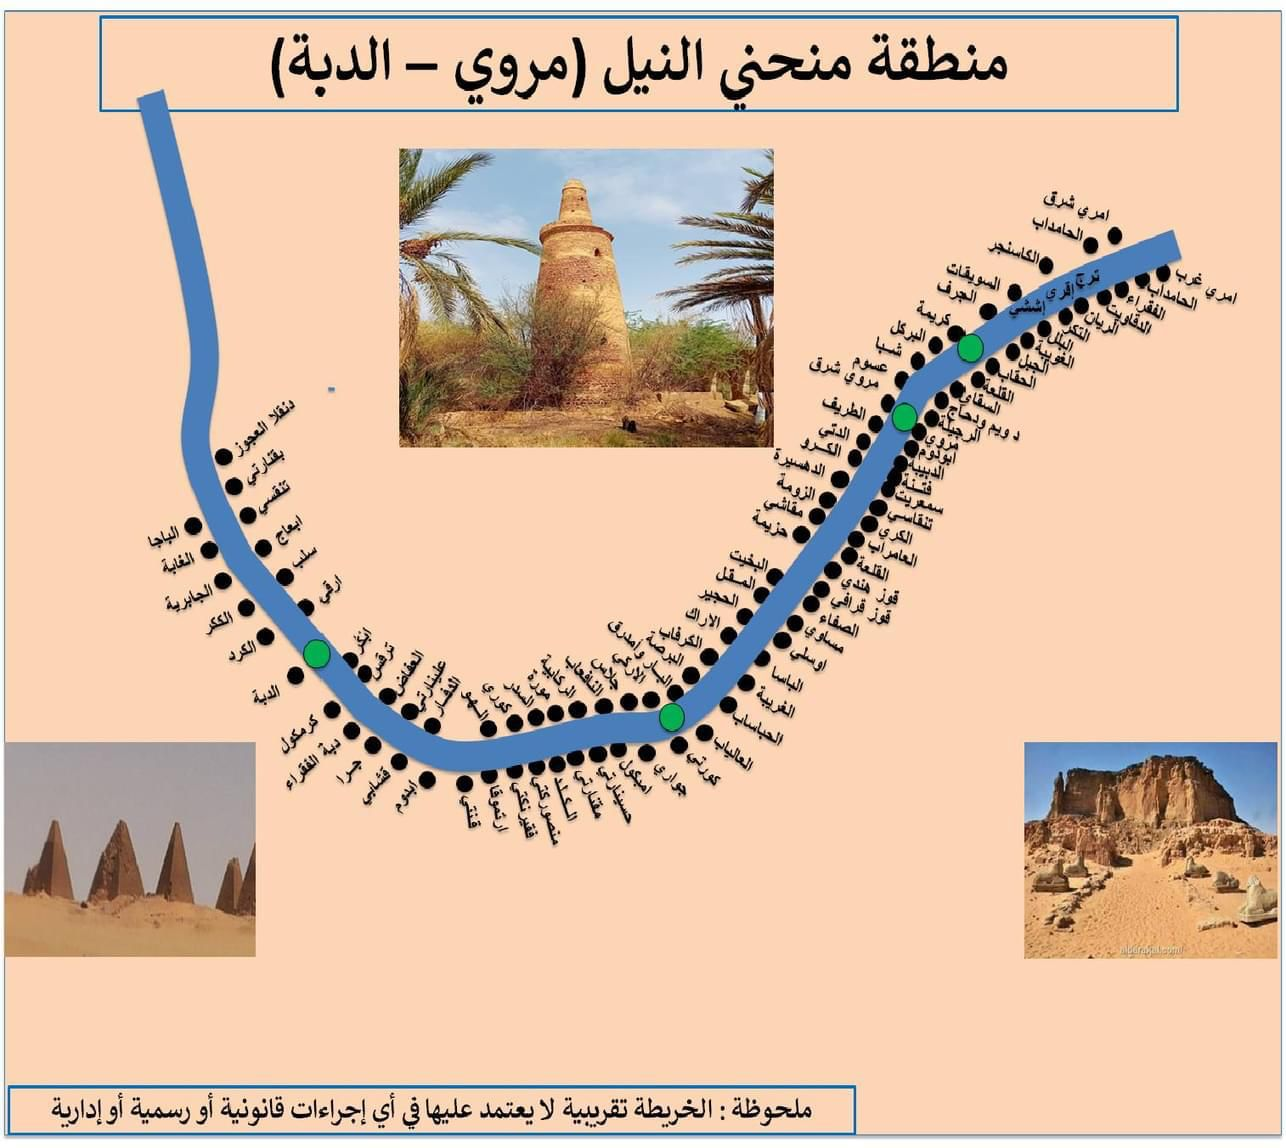
\includegraphics[width=0.4\textwidth]{120.jpg}
\end{wrapfigure}

\end{document}




